
%(BEGIN_QUESTION)
% Copyright 2010, Tony R. Kuphaldt, released under the Creative Commons Attribution License (v 1.0)
% This means you may do almost anything with this work of mine, so long as you give me proper credit

A researcher builds an experimental hot-air solar collector with a loop controller to maintain a constant interior temperature regardless of solar input:

$$\includegraphics[width=15.5cm]{i01417x01.eps}$$

The researcher also wishes to graph the temperature and fan command signals (PV and Output) using a data acquisition module (DAQ) connecting to a personal computer.  The DAQ is capable of measuring DC voltage signals ranging from 0 to +7.5 volts (single-ended), like a four-channel DC voltmeter sharing a common negative terminal.

\vskip 10pt

Sketch the necessary connecting wires to allow this DAQ unit to measure the temperature signal on input Ain2 and the fan command signal on input Ain0.

\vfil 

\underbar{file i01417}
\eject
%(END_QUESTION)





%(BEGIN_ANSWER)

This is a graded question -- no answers or hints given!
 
%(END_ANSWER)





%(BEGIN_NOTES)

The fact that the DAQ has one common negative terminal for all four of its inputs, plus the fact that both the controller's PV input and Output share a common ground, makes it possible to measure these two data points using only three wires between the controller and DAQ:

$$\includegraphics[width=15.5cm]{i01417x02.eps}$$

Alternatively, the ``Gnd'' terminal on the DAQ could be connected to the ($-$) terminal of the PV input rather than the ($-$) terminal of the controller Output.

%INDEX% Pictorial circuit review (analog signal wiring to data acquisition unit)

%(END_NOTES)


